\subsection{a)}

\begin{equation}
K_c>\frac{b}{a(b-c)}
\end{equation}
\subsection{b)}


\begin{equation}
c_s>\sqrt{4D(b-c)} \Rightarrow c_s>\sqrt{2}
\end{equation}

\subsection{c)}

\begin{figure}[h]
    \centering
    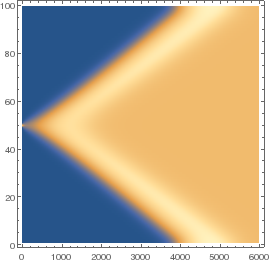
\includegraphics[width=0.45\textwidth]{img/listdensityplot_S.eps}
    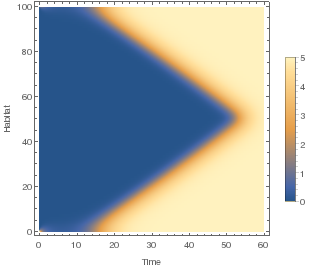
\includegraphics[width=0.45\textwidth]{img/listdensityplot_P.eps}
  \caption{}
\end{figure}
